\let\negmedspace\undefined
\let\negthickspace\undefined
\documentclass[journal]{IEEEtran}
\usepackage[a5paper, margin=10mm, onecolumn]{geometry}
%\usepackage{lmodern} % Ensure lmodern is loaded for pdflatex
\usepackage{tfrupee} % Include tfrupee package

\setlength{\headheight}{1cm} % Set the height of the header box
\setlength{\headsep}{0mm}     % Set the distance between the header box and the top of the text

\usepackage{gvv-book}
\usepackage{gvv}
\usepackage{cite}
\usepackage{amsmath,amssymb,amsfonts,amsthm}
\usepackage{algorithmic}
\usepackage{graphicx}
\usepackage{textcomp}
\usepackage{xcolor}
\usepackage{txfonts}
\usepackage{listings}
\usepackage{enumitem}
\usepackage{mathtools}
\usepackage{gensymb}
\usepackage{comment}
\usepackage[breaklinks=true]{hyperref}
\usepackage{tkz-euclide} 
\usepackage{listings}
% \usepackage{gvv}                                        
\def\inputGnumericTable{}                                 
\usepackage[latin1]{inputenc}                                
\usepackage{color}                                            
\usepackage{array}                                            
\usepackage{longtable}                                       
\usepackage{calc}                                             
\usepackage{multirow}                                         
\usepackage{hhline}                                           
\usepackage{ifthen}                                           
\usepackage{lscape}
\begin{document}

\bibliographystyle{IEEEtran}
\vspace{3cm}

\title{2013-AE-27-39}
\author{EE24BTECH11066 - YERRA AKHILESH
}
% \maketitle
% \newpage
% \bigskip
{\let\newpage\relax\maketitle}

\renewcommand{\thefigure}{\theenumi}
\renewcommand{\thetable}{\theenumi}
\setlength{\intextsep}{10pt} % Space between text and floats


\numberwithin{equation}{enumi}
\numberwithin{figure}{enumi}
\renewcommand{\thetable}{\theenumi}
\begin{enumerate}[start=27]
\item Given that the Laplace transform, $\mathcal{L}\brak{e^{at}}=\frac{1}{s-a}$ then $\mathcal{L}\brak{3e^{5t \sinh{5t}}}=$ \hfill{[2013-AE]}
\begin{enumerate}
\begin{multicols}{4}
\item $\frac{3s}{s^2-10s}$
\item $\frac{15}{s^2-10s}$
\item $\frac{3s}{s^2+10s}$
\item $\frac{15}{s^2+10s}$
\end{multicols}
\end{enumerate}
%28
\item Values of $a,b \text{ and } c$, which render the matrix\\
$Q=\myvec{\frac{1}{\sqrt{3}}&\frac{1}{\sqrt{2}}&a\\ \frac{1}{\sqrt{3}}&0&b\\ \frac{1}{\sqrt{3}}&\frac{-1}{\sqrt{2}}&c}$\\
orthonormal are, respectively \hfill{[2013-AE]}
\begin{enumerate}
    \item $\frac{1}{\sqrt{2}},\frac{1}{\sqrt{2}}.0$\\
    \item $\frac{1}{\sqrt{6}},\frac{-2}{\sqrt{6}},\frac{1}{\sqrt{6}}$\\
    \item $\frac{-1}{\sqrt{3}},\frac{-1}{\sqrt{3}},\frac{1}{\sqrt{3}}$\\
    \item $\frac{-1}{\sqrt{6}},\frac{2}{\sqrt{6}},\frac{-1}{\sqrt{6}}$
\end{enumerate}
%29
\item  A function $y(t)$ satisfies the differential equation $\frac{d^2 y}{dt^2}-2\frac{dy}{dt}+y=0$ and is subject to the initial conditions $y\brak{t=0}=0$ and $\frac{dy}{dt}\brak{t=0}=1$. The value of $y\brak{t=1}$ is \hfill{[2013-AE]}
\begin{enumerate}
\begin{multicols}{4}
\item $e$
\item 0
\item 1
\item -1
\end{multicols}
\end{enumerate}
%30
\item A glider is launched from a $500m$ high hilltop. Following data is available for the glider: Zero lift drag coefficient $C_{D0}=0.02$, aspect ratio $AR=10$ and Oswald efficiency factor $e=0.95$. The maximum range of the glider in km is \underline{\hspace{1cm}}\\

    \hfill{[2013-AE]}
%31
\item Which one of the following criteria leads to maximum turn rate and minimum radius in a level turn flight? \hfill{[2013-AE]}
\begin{enumerate}
    \item Highest possible load factor and highest possible velocity
    \item Lowest possible load factor and lowest possible velocity
    \item Highest possible load factor and lowest possible velocity
    \item Lowest possible load factor and highest possible velocity
\end{enumerate}
%32
\item Consider an airplane with a rectangular straight wing at dihedral angle $\Gamma = 10^{\circ}$. The lift curve slope of the wing airfoil section $\brak{\text{constant over the whole span of the wing}}$ is $c_{l \alpha} = \frac{5.4}{\text{rad}}$. The roll stability derivative, $C_{l \beta}$ in per radian is \underline{\hspace{1cm}} \hfill{[2013-AE]}\\
%33
\item Consider one-dimensional isentropic flow at a Mach number of $0.5$. If the area of cross-section of a streamtube increases by $3\%$ somewhere along the flow, the corresponding percentage change in density is \underline{\hspace{1cm}} \hfill{[2013-AE]}\\
%34
\item The potential flow model for a storm is represented by the superposition of a sink and a vortex. The stream function can be written in the $\brak{r,\theta}$ system as $\psi=\frac{\Lambda}{2\pi}\theta+\frac{\Gamma}{2\pi} \text{ln } r$, where $\Lambda=\Gamma=100 \frac{m^2}{s}$.Assume a constant air density of $1.2 \frac{kg}{m^3}$. The gauge pressure at a distance of $100 m$ from the storm eye is \hfill{[2013-AE]}
\begin{enumerate}
\begin{multicols}{4}
\item $-\infty$
\item $\frac{-1.2}{\pi ^2}$
\item $\frac{-1.2}{2\pi ^2}$
\item $\frac{-1.2}{4\pi ^2}$
\end{multicols}
\end{enumerate}
%35
\item Three identical eagles of wing span $s$ are flying side by side in a straight line with no gap between their wing tips. Assume a single horse shoe vortex model $\brak{\text{of equal strength}\Gamma}$ for each bird. The net downwash experienced by the middle bird is \hfill{[2013-AE]}
\begin{enumerate}
\begin{multicols}{4}
\item $\frac{\Gamma}{\pi s}$
\item $\frac{\Gamma}{2\pi s}$
\item $\frac{\Gamma}{3\pi s}$
\item $\frac{4\Gamma}{3\pi s}$
\end{multicols}
\end{enumerate}
%36
\item Streamline pattern of flow past a cylinder is shown in the figure below. The oncoming flow is steady, irrotational and incompressible. The flow is from left to right. Bernoulli's equation CANNOT be applied between the points \hfill{[2013-AE]}\\
\begin{figure}[h!]
    \centering
    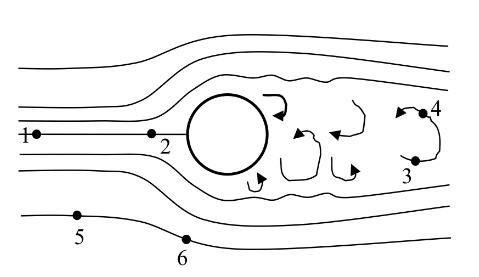
\includegraphics[width=0.5\linewidth]{figs/Figure_2.png}
    \label{fig:enter-label}
\end{figure}
\begin{enumerate}
\begin{multicols}{4}
\item 1 and 2
\item 1 and 5
\item 3 and 4
\item 5 and 6
\end{multicols}
\end{enumerate}
%37
\item Consider a supersonic stream at a Mach number $M=2$, undergoing a gradual expansion. The stream is turned by an angle of $3$ degrees due to the expansion. The following data is given.\\
\begin{table}[H]    
  \centering
  \begin{tabular}[12pt]{ |c| c|}
    \hline
    \textbf{M} & $\nu$ \textbf{(Prandtl-Meyer function)}\\ 
    \hline
    1.8 & 20.73 \\
    \hline
    1.9 & 23.59 \\
    \hline
    2.0 & 26.38 \\
    \hline
    2.1 & 29.10 \\
    \hline
    2.2 & 31.73 \\
    \hline
    2.3 & 34.28 \\
    \hline
    2.4 & 36.75 \\
    \hline
    \end{tabular}
  \label{tab1-1.8-10}
\end{table}
The Mach number downstream of the expansion is \hfill{[2013-AE]}
\begin{enumerate}
\begin{multicols}{4}
\item $1.88$
\item $2.00$
\item $2.11$
\item $2.33$
\end{multicols}
\end{enumerate}
%38
\item The idealized cross-section of a beam is comprised of four identical booms connected by shear webs. The beam is subjected to a bending moment $M$ as shown in the figure. The inclination of the neutral axis to the x-axis in degrees is \hfill{[2013-AE]}
\begin{figure}[H]
    \centering
    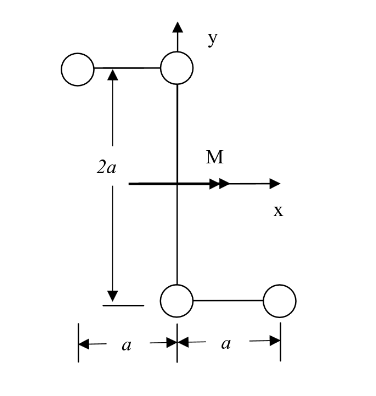
\includegraphics[width=0.5\linewidth]{figs/Figure_3.png}
    \label{fig:enter-label}
\end{figure}
\begin{enumerate}
\begin{multicols}{4}
\item $45$ CW
\item $45$ CCW
\item $26.6$ CW
\item $63.4$ CCW
\end{multicols}
\end{enumerate}
%39
\item A composite circular shaft is comprised of a steel core surrounded by an aluminum annulus, perfectly bonded to each other as shown in the figure. If it subjected to a pure torque, which one of the following statements is TRUE? \hfill{[2013-AE]}
\begin{figure}[H]
    \centering
    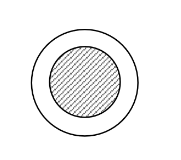
\includegraphics[width=0.5\linewidth]{figs/Figure_1.png}
    \label{fig:enter-label}
\end{figure}
\begin{enumerate}
    \item Only shear stress is continuous across the steel-aluminum interface
    \item Only shear strain is continuous across the steel-aluminum interface
    \item Both shear stress and shear strain are continuous across the steel-aluminum interface
    \item Both shear stress and shear strain are discontinuous across the steel-aluminum interface
\end{enumerate}
\end{enumerate}
\end{document}

